%Nervous systems in animals are different, from the simple ones found in insects to more complex ones in reptiles, birds and mammals. They are all composed mainly of a special kind of cell, the \emph{ neuron}, that excels at long distance communication. Most animal's nervous systems include an organ called the \emph{brain} which plays a central role on the everyday life of the animal. In most cases the brain will be located in the head which is the closest location to the primary sensing organs like eyes, tongue or ears~\cite{scholarpedia-brain}.\\


Studies have found that the brain is formed by many components~\cite{thompson2000brain}, a brief description of the principal parts (shown in Figure \ref{fig:brain:components}) is presented next. 
\begin{description}
  \item[The cortex] is a wrinkled sheet of neurons that's the largest portion of the brain and is responsible for high level cognition, motor control, memory and problem solving, to name a few.
  \item[The cerebellum,] also known as the ``small brain'' is mostly involved in sensorimotor tasks like balance or the coordination of the body.
  \item[The brain stem,] which is located under the cerebrum and in front of the cerebellum, it connects the brain to the spinal cord and is in charge of automatic functions like breathing or digestion.
  \item[The limbic System,] it had been thought of as the ``old brain'' sits between the brain stem and the cortex. Some of its functions include hormonal control, emotions, learning and memory consolidation. A particular section of the limbic system is known as the \emph{hippocampus}, it plays a major role in memory and spatial location and will be described in Section \ref{sec:brain:hippo}.
\end{description}

\begin{figure}[hbt]
  \begin{center}
    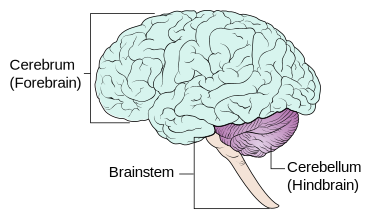
\includegraphics[width=0.6\textwidth]{Diagram_showing_some_of_the_main_areas_of_the_brain_CRUK_188}
    \caption{Main areas of the brain~\cite{wikipedia-images}.}
    \label{fig:brain:components}
  \end{center}
  
\end{figure}

About 80\% of the neurons in the brain are located inside the cortex. This thin sheet of about 1100 $cm^2$ area and a 2 to $4 mm$ thickness is responsible for the high-level cognitive tasks humans can perform~\cite{thompson2000brain}. It makes us capable of the most diverse behaviours, from reading this report to cooking or running a marathon, the cortex is the motor behind our thoughts. 

The fact that the cortex is thoroughly wrinkled allows a larger area sheet, and thus neurons, to fit in the same volume. It is composed of two symmetric shapes, the left and right \emph{hemispheres} (left of Figure~\ref{fig:brain:hemi-lobes}). Although both share functions, it has been observed that one hemisphere may dominate the other on some tasks~\cite{lateralization}. 

\begin{figure}[hbt]
  \begin{center}
    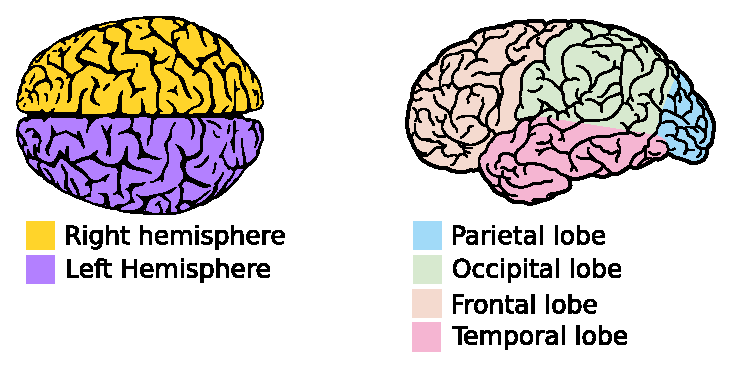
\includegraphics[width=0.7\textwidth]{human_brain_lobes}
    \caption{Left: The left and right brain hemispheres. Right: The brain divided into lobes.}
    \label{fig:brain:hemi-lobes}
  \end{center}
\end{figure}

Anatomists have divided the cortex into regions, known as \emph{lobes},  separated by large creases (right of Figure~\ref{fig:brain:hemi-lobes}). New classification of areas are constantly being discovered, whose class ranges from the functional to the physiological~\cite{eye-brain-vision-hubel1995}. Some areas that most scientists agree on are the somatosensory cortex, that deals with touch; and the striate cortex, which plays a role in visual perception (more on this in Chapter \ref{chp:vision}).

\begin{figure}[ht]
  \begin{center}
    \begin{subfigure}{0.4\textwidth}
      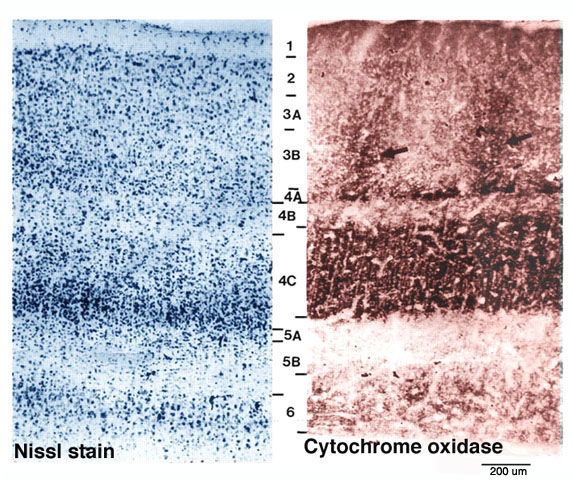
\includegraphics[width=\textwidth]{Nissl-CO}
      \caption{Stained samples}
    \end{subfigure}
    \begin{subfigure}{0.4\textwidth}
      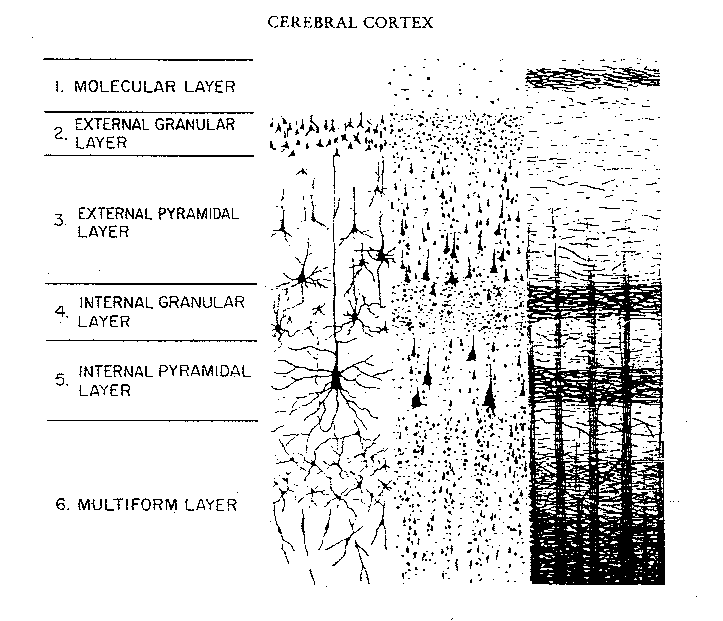
\includegraphics[width=\textwidth]{FigV5}
      \caption{Diagram of cell types, distribution of cells, and connectivity.}
    \end{subfigure}
    \caption{Cerebral cortex sections showing layered organization.}
    \label{fig:neuro:cortex-layers}
  \end{center}
\end{figure}

Cell distribution in the cortex seems to follow a pattern, as seen in Figure~\ref{fig:neuro:cortex-layers}. If a section is taken from it,  layers can be observed and it they are thought to have special functions; some  receive input (usually layer 4) from other parts of the brain and/or output (layers 2,3,5 and 6) connections to other areas~\cite{thompson2000brain,eye-brain-vision-hubel1995}. This organization forms a cortical microcircuit, which is thought to be the basic building block of cortical functions.
%Although some connectivity is known, the actual function of these layers is still a matter of research.

